\documentclass[11pt,a4paper]{article}
\usepackage[utf8]{inputenc}\usepackage[T1]{fontenc}\IfFileExists{italian.ldf}{\usepackage[italian]{babel}}{\usepackage[english]{babel}}\usepackage{amsmath,amssymb,amsthm,geometry,tikz}\geometry{margin=2cm}
\newcommand{\R}{\mathbb R}\newcommand{\F}{\mathbb F}\newcommand{\tr}{\operatorname{tr}}\newcommand{\ar}{\operatorname{arr}}\newcommand{\fl}{\operatorname{fl}}
\newcommand{\pagina}[1]{\clearpage}
\begin{document}\title{Calcolo numerico}\author{Trascrizione degli appunti}\date{}\maketitle
% Pagina originale 1
\section*{Legenda}
\begin{enumerate}
\item \textbf{Numeri macchina}
\begin{itemize}
\item Rappresentazione numerica
\item Distanza
\item Underflow
\item Overflow
\item Troncamento
\item Arrotondamento
\item Operazioni tra numeri macchina
\item Proprietà operazioni macchina
\end{itemize}
\item \textbf{Equazioni non lineari}
\begin{itemize}
\item Th. degli zeri
\item Metodo di bisezione
\item Metodo della falsa posizione
\item Metodi di iterazione funzionale
\item Interpretazione geometrica
\item Convergenza locale
\item Criterio di stop
\item Ordine di convergenza
\item Metodo di Newton-Raphson
\item Th. convergenza
\item Molteplicità di una radice
\item Metodo della direzione costante
\item Metodo della secante
\end{itemize}
\item \textbf{Sistemi di equazioni lineari}
\begin{itemize}
\item Regola di Cramer
\item Metodo di eliminazione di Gauss
\item Strategie di pivoting
\item Pivoting parziale
\item Pivoting totale
\item Fattorizzazione LU
\item Equivalenza tra Gauss e LU
\item Condizionamento sistemi lineari
\end{itemize}
\item \textbf{Interpolazione}
\begin{itemize}
\item Interpolazione polinomiale
\item Polinomio interpolante di Lagrange
\item Errori di interpolazione
\item Th. di rappresentazione dell’errore di interpolazione
\item Fenomeno di Runge
\item Minimizzare il resto nel problema di interpolazione
\item Polinomio di Chebyshev
\item Th. di Minimax
\item Funzioni spline
\item Approssimazione ai minimi quadrati
\item Retta di regressione
\end{itemize}
\item \textbf{Quadratura}
\begin{itemize}
\item Formule di quadratura di tipo interpolatorio
\item Grado di precisione
\item Formula di Newton-Cotes
\item Formula dei Trapezi
\item Resto nella formula dei trapezi
\item Th. della media generalizzato
\item Formula di Simpson
\item Formula del punto di mezzo
\item Formule di quadratura composta
\item Formula dei trapezi composta
\item Formula di Simpson composta
\item Formula del punto di mezzo composta
\end{itemize}
\item \textbf{Derivazione numerica}
\begin{itemize}
\item Differenze in avanti
\item Differenze all’indietro
\end{itemize}
\item \textbf{Eq. differenziali}
\begin{itemize}
\item Metodo di Eulero esplicito
\item Metodo di Eulero implicito
\item Metodo dei trapezi
\item Metodo del midpoint
\item Classificazione metodi numerici
\item Studio della convergenza
\end{itemize}
\end{enumerate}
% Pagina originale 2
\pagina{2}\section{Numeri macchina}
Il calcolo numerico è una branca della matematica che cerca di risolvere problemi matematici utilizzando uno o più algoritmi. Il computer ha una memoria finita e questo porta ad approssimazioni di numeri e risultati. Le approssimazioni sono sinonimi di errore. Gli errori possono essere analitici (dovuti all'esigenza di calcolare sommatorie infinite in un tempo finito) o di rappresentazione (dovuti all'esigenza di rappresentare un numero con infinite cifre in una memoria finita).
È possibile misurare l'errore in due modi:
\[e_A(x)=\|x-\widetilde x\|,\qquad e_R(x)=\frac{\|x-\widetilde x\|}{\|x\|},\quad x\ne0.\]
\subsection*{Rappresentazione numerica}
Rappresentare $\R$ diventa impossibile. Viene utilizzato un insieme $\F$ dei floating point numbers. Si utilizza la rappresentazione normalizzata, cioè parte intera nulla e prima cifra dopo la virgola non nulla:
\[x=(-1)^s\,0.d_1d_2\cdots d_t\,\beta^E,\quad d_1\ne0.\]
\[\F(\beta,t,m,M)=\{x\in\R:x=(-1)^s0.d_1\cdots d_t\beta^E\}\cup\{0\},\]
con $t\ge1$, $\beta\ge2$, $m,M>0$, $d_1\ne0$, $d_i\in\{0,\ldots,\beta-1\}$, $E\in[-m,M]$. $\beta$ è la base, $t$ il numero di cifre della mantissa, $m$ il valore assoluto dell'esponente minimo, $M$ l'esponente massimo.
% Pagina originale 3
\pagina{3}
Un bit per il segno $s$, $t$ bit per la mantissa $(d_1,\ldots,d_t)$, $M+m+1$ combinazioni per l'esponente $E$.
I numeri macchina hanno varie proprietà: $\F$ è discreto; i numeri rappresentabili sono solo una piccola parte di $\R$; la distanza tra due numeri consecutivi non è costante.
\[x_i=\beta^E0.d_1\cdots d_{t-1}d_t,\quad x_{i+1}=\beta^E0.d_1\cdots d_{t-1}\widetilde d_t,\quad\widetilde d_t=d_t+1.\]
La distanza è $x_{i+1}-x_i=\beta^E0.00\cdots1=\beta^{E-t}$. Per $E=-m$ vale $\beta^{-m-t}$; per $E=M$ vale $\beta^{M-t}$. Il rapporto tra le distanze è $\beta^{M+m}$ (enorme).
\subsection*{Underflow e overflow}
Ci sono numeri troppo vicini allo zero per essere rappresentati e numeri troppo grandi. Se
\[x=\pm\beta^E\sum_{i=1}^{n}d_i\beta^{-i},\quad n\le t,\ E<-m,\]
il numero è più piccolo del più piccolo elemento positivo di $\F$ e si verifica underflow.
% Pagina originale 4
\pagina{4}
Se $x<\min\F^+$, $x$ sarà calcolato come zero. Se $x=\pm\beta^E\sum_{i=1}^n d_i\beta^{-i}$, $n\le t$, $E>M$, il numero è più grande del massimo elemento di $\F$ e si verifica overflow. Se $x>\max\F$, $x$ sarà considerato $\mathrm{Inf}$.
\subsection*{Troncamento e arrotondamento}
Se $n>t$, bisognerà troncare il numero per poterlo rappresentare:
\[\widetilde x=\tr(x)=\pm\beta^E\sum_{i=1}^t d_i\beta^{-i},\]
\[\widehat x=\ar(x)=\pm\left(\beta^E\sum_{i=1}^t d_i\beta^{-i}+\Omega\beta^{E-t}\right),\quad\Omega=\begin{cases}0&d_{t+1}<\beta/2,\\1&d_{t+1}\ge\beta/2.\end{cases}\]
Se $x\notin\F$, esistono $a,b\in\F$ tali che $a\le x\le b$. Se $x<(a+b)/2$, $a=\tr(x)=\ar(x)$; se $x\ge(a+b)/2$, $a=\tr(x)$ e $b=\ar(x)$.
L'arrotondamento può portare all'overflow, anche all'underflow. Se $d_i=\beta-1$ per ogni $i=1,\ldots,t$, $E=M$ e $d_{t+1}\ge\beta/2$, allora $\ar(x)=\pm\beta^M=\pm0.1\beta^{M+1}$. Troncamento e arrotondamento producono errori.
% Pagina originale 5
\pagina{5}
Calcoliamo l'errore di trasformazione:
\[|\tr(x)-x|<b-a=\beta^{E-t},\quad |x|=\beta^E0.d_1\cdots d_t\ge\beta^{E-1}.\]
\[e_R(x)=\frac{|x-\tr(x)|}{|x|}\le\beta^{1-t}.\]
\[|\ar(x)-x|\le\tfrac12(b-a)=\tfrac12\beta^{E-t},\qquad e_R(x)\le\tfrac12\beta^{1-t}.\]
I numeri $u<\beta^{1-t}$ sono detti zero macchina per il troncamento ($u<\frac12\beta^{1-t}$ per l'arrotondamento). Posto $\varepsilon_x=(\widetilde x-x)/x$, con $|\varepsilon_x|\le u$, segue $\widetilde x=x(1+\varepsilon_x)$. È la relazione tra $x\in\R$ e $\widetilde x=\fl(x)\in\F$.
\subsection*{Operazioni tra numeri macchina}
$x,y\in\F$ non implica $x\cdot y\in\F$. L'operazione macchina soddisfa
\[x\odot y=(x\cdot y)(1+\varepsilon),\quad |\varepsilon|<u.\tag{1}\]
$x\cdot y=x\odot y$ se e solo se $\varepsilon=0$. Le operazioni $\tr(x\cdot y)$ o $\ar(x\cdot y)$ soddisfano (1). Ogni operazione ha un metodo per essere effettuata correttamente.
% Pagina originale 6
\pagina{6}
\subsection*{Addizione e sottrazione (somma algebrica)}
Siano $x,y\in\F(\beta,t,m,M)$. I passaggi sono:
\begin{enumerate}\item Prendere l'esponente maggiore e modificare il numero con esponente minore affinché $E_y=E_x$.\item Sommare le mantisse.\item Normalizzare la somma delle mantisse.\item Arrotondare o troncare il risultato.\end{enumerate}
Esempio: $x=0.78546\cdot10^2$, $y=0.61332\cdot10^{-1}$, $\widetilde y=0.00061\cdot10^2$, $x\oplus y=0.78607\cdot10^2$.
Esempio: $x\simeq y$, $x=0.75868531\cdot10^2$, $y=0.75868100\cdot10^2$. $\widetilde x=0.75869\cdot10^2$, $\widetilde y=0.75868\cdot10^2$.
\[\fl(\widetilde x-\widetilde y)=0.00001\cdot10^2=0.1\cdot10^{-2},\]
\[x-y=0.00000431\cdot10^2=4.31\cdot10^{-4}=0.0431\cdot10^{-2}.\]
\[e_R(x-y)=\frac{|\fl(\widetilde x-\widetilde y)-(x-y)|}{|x-y|}\simeq1.32.\]
Errore molto elevato: cancellazione numerica di cifre significative quando $x\simeq y$.
% Pagina originale 7
\pagina{7}
La cancellazione numerica di cifre significative rappresenta un caso di problema mal condizionato.
\subsection*{Prodotto}
\[x\odot y=\ar(\operatorname{mantissa}(x)\operatorname{mantissa}(y))\beta^{E_x+E_y}.\]
I passaggi: eseguire il prodotto delle mantisse; arrotondare/troncare le $t$ cifre dopo aver normalizzato; moltiplicare per $\beta^{E_x+E_y}$ (sommare gli esponenti).
Esempio: $x=0.11111\cdot10^3$, $y=0.52521\cdot10^2$:
\[0.11111\cdot0.52521=0.05835608\simeq0.58356\cdot10^{-1},\quad x\odot y=0.58356\cdot10^4.\]
\subsection*{Divisione}
Scalare l'esponente di $x$ affinché $\operatorname{mantissa}(x)<\operatorname{mantissa}(y)$; dividere le mantisse; normalizzare e arrotondare/troncare; sottrarre gli esponenti.
Esempio: $x=0.12100\cdot10^5$, $y=0.11000\cdot10^2$, $\widetilde x=0.01210\cdot10^6$. Il rapporto delle mantisse è $0.11000$ e $x\oslash y=0.11000\cdot10^{6-2}=0.11000\cdot10^4$.
% Pagina originale 8
\pagina{8}
\subsection*{Proprietà delle operazioni macchina}
\begin{enumerate}\item $\F$ non è chiuso rispetto alle operazioni macchina (a causa dell'underflow).\item L'elemento neutro per la somma non è unico: numeri molto piccoli vengono considerati zero.\item L'elemento neutro per il prodotto non è unico: numeri molto vicini a uno.\item Non vale l'associatività di somma e prodotto: $(a+b)+c\ne a+(b+c)$.\item Non vale la distributività: $a(b+c)\ne ab+ac$.\end{enumerate}
\subsection*{Condizionamento dei problemi}
Un problema si dice ben condizionato se a piccoli errori sui dati corrispondono piccoli errori sui risultati. È mal condizionato se non è ben condizionato. Il condizionamento è una caratteristica intrinseca del problema e non dipende dal metodo di risoluzione adottato. Un problema mal condizionato va sostituito con uno meglio condizionato tramite tecniche di precondizionamento.
% Pagina originale 9
\pagina{9}\section{Equazioni non lineari}
\subsection*{Teorema degli zeri}
Sia $f:[a,b]\to\R$, $f\in C([a,b])$, $f(a)f(b)<0$. Allora esiste $c\in(a,b)$ tale che $f(c)=0$.
\subsection*{Metodo di bisezione}
Si costruisce una successione di intervalli $\{I_k\}_{k=0}^\infty$ tale che $I_0=[a,b]$, $I_{n+1}\subset I_n$, $\alpha\in I_n$ per ogni $n\ge0$ e $|I_k|\to0$ per $k\to\infty$.
$I_0=[a_0,b_0]$, $c_1=(a_0+b_0)/2$. Se $f(a)f(c)<0$, $a_1=a_0$, $b_1=c_1$; se $f(c)f(b)<0$, $a_1=c_1$, $b_1=b_0$. In generale
\[c_{k+1}=\frac{a_k+b_k}{2}.\]
Se $f(c_k)=0$, $c_k=\alpha$, zero di $f$. A causa degli errori di arrotondamento la condizione $f(c_k)=0$ non viene quasi mai verificata. Bisogna stabilire un criterio di stop, per esempio $b_k-a_k\le\varepsilon$, con tolleranza prefissata.
% Pagina originale 10
\pagina{10}
Scelta una tolleranza prefissata, si può dedurre il numero di passi:
\[b_k-a_k=\frac{b_0-a_0}{2^k}\le\varepsilon\quad\Longrightarrow\quad k\ge\log_2\frac{b_0-a_0}{\varepsilon}.\]
Se $0\notin[a,b]$, un altro criterio è
\[\frac{b_k-a_k}{\min(|a_k|,|b_k|)}\le\varepsilon\quad\text{(errore relativo)},\]
mentre $b_k-a_k\le\varepsilon$ controlla l'errore assoluto. Un altro criterio potrebbe essere $|f(c_k)|\le\varepsilon$.
\subsection*{Metodo della falsa posizione}
La retta secante è
\[y=f(a)+\frac{f(b)-f(a)}{b-a}(x-a).\]
Ponendo $y=0$ si ottiene
\[c_1=a-f(a)\frac{b-a}{f(b)-f(a)}.\]
Se $f(a_0)f(c_1)<0$ si pone $a_1=a_0,b_1=c_1$; se $f(a_0)f(c_1)>0$, $a_1=c_1,b_1=b_0$. Il metodo è uguale alla bisezione, ma cambia il calcolo di $c_k$. Entrambi hanno vantaggi e svantaggi.
% Pagina originale 11
\pagina{11}
Vantaggi: richiedono esclusivamente la continuità di $f$; possono ricavare buone approssimazioni di $\alpha$, usabili come starting point per metodi iterativi. Svantaggi: convergenza lenta (una cifra di precisione in base due per passo); velocità di convergenza indipendente da $f$.
\subsection*{Metodi di iterazione funzionale}
Sono metodi $x_{k+1}=g(x_k)$, $k=0,1,\ldots$, dove $x_0$ è uno starting point. Ogni punto $\alpha$ tale che $g(\alpha)=\alpha$ è un punto fisso di $g$; $g$ è detta funzione iteratrice. Per trovare gli zeri di una funzione si può definire
\[g(x)=x-\frac{f(x)}{h(x)},\quad h:[a,b]\to\R\setminus\{0\}.\]
Infatti $g(\alpha)=\alpha-f(\alpha)/h(\alpha)=\alpha$ se e solo se $f(\alpha)=0$.
\textbf{Teorema.} Se $g\in C([a,b])$, la successione $x_{k+1}=g(x_k)$ è contenuta in $[a,b]$ e converge, il suo limite $\alpha$ soddisfa $g(\alpha)=\alpha$.
\textit{Dimostrazione.} $\alpha=\lim x_{k+1}=\lim g(x_k)=g(\lim x_k)=g(\alpha)$.
% Pagina originale 12
\pagina{12}
Questa è una condizione necessaria ma non sufficiente.
\textbf{Teorema (condizione sufficiente).} Sia $\alpha$ punto fisso e $g\in C^1([\alpha-\rho,\alpha+\rho])$, $\rho>0$. Se $|g'(x)|<1$ su tale intervallo, allora: per ogni $x_0$ nell'intervallo, anche tutti gli $x_k$ vi appartengono; $x_k\to\alpha$; $\alpha$ è l'unico punto fisso nell'intervallo.
La condizione garantisce unicità, convergenza e permanenza nell'intervallo.
\subsection*{Interpretazione geometrica}
Si alternano il grafico $y=g(x)$ e la retta $y=x$: $x_1=g(x_0)$, $x_2=g(x_1)$, eccetera. Nel caso rappresentato $g'(x)\in(-1,0)$ e gli iterati oscillano attorno al punto fisso.
\subsection*{Convergenza locale}
Un metodo iterativo è localmente convergente per $\bar\alpha=g(\bar\alpha)$ se esiste $[a,b]$ tale che per ogni $x_0\in[a,b]$ la successione converge a $\bar\alpha$. Spostando anche di poco $x_0$ si potrebbe trovare un punto fisso diverso o non trovarne alcuno.
% Pagina originale 13
\pagina{13}
\subsection*{Criteri di stop}
$e_k(\alpha)=|\alpha-x_k|<\varepsilon$ non è verificabile, non conoscendo $\alpha$. Criteri validi possono essere
\[|x_{k+1}-x_k|\le\varepsilon,\quad\frac{|x_{k+1}-x_k|}{\min(|x_{k+1}|,|x_k|)}\le\varepsilon,\quad |f(x_k)|\le\varepsilon.\]
\subsection*{Ordine di convergenza}
Sia $x_k\to\alpha$, $x_k\ne\alpha$ per ogni $k$. Se esiste $p\ge1$ tale che
\[\lim_{k\to\infty}\frac{|x_{k+1}-\alpha|}{|x_k-\alpha|^p}=\gamma,\]
con $0\le\gamma\le1$ per $p=1$ e $\gamma>0$ per $p>1$, la successione ha ordine $p$ e $\gamma$ è la costante asintotica di convergenza. Per $p=1$, $\gamma\in(0,1)$, la convergenza è lineare; $p>1$ superlineare; $p=2$ quadratica; $p=3$ cubica.
Esiste $\beta\simeq\gamma$ tale che
\[|x_{k+1}-\alpha|\le\beta|x_k-\alpha|^p,\quad\frac{|x_{k+1}-\alpha|}{|\alpha|}\le\beta|\alpha|^{p-1}\left|\frac{x_k-\alpha}{\alpha}\right|^p.\]
Quindi $e^A_{k+1}\le\beta(e^A_k)^p$ ed $e^R_{k+1}\le\beta|\alpha|^{p-1}(e^R_k)^p$.
% Pagina originale 14
\pagina{14}
\textbf{Teorema.} Per $x_{k+1}=g(x_k)\to\alpha=g(\alpha)$, $g\in C^{p+1}(I(\alpha,\rho))$, l'ordine è $p\ge1$ se e solo se
\[g'(\alpha)=\cdots=g^{(p-1)}(\alpha)=0,\quad g^{(p)}(\alpha)\ne0,\quad\gamma=\frac{|g^{(p)}(\alpha)|}{p!}.\]
\subsection*{Metodo di Newton--Raphson}
È chiamato metodo delle tangenti; richiede $f\in C^1([a,b])$. La tangente in $x_k$ è $y-f(x_k)=f'(x_k)(x-x_k)$. Ponendo $y=0$:
\[x_{k+1}=x_k-\frac{f(x_k)}{f'(x_k)}.\]
Si tratta della precedente iterazione con $h(x)=f'(x)$.
\textbf{Teorema di convergenza.} Sia $f\in C^3([a,b])$, $f'(x)\ne0$ per ogni $x\in[a,b]$, $\alpha\in[a,b]$ zero di $f$. Esiste $[\alpha-\rho,\alpha+\rho]$ tale che ogni iterazione iniziata al suo interno converge ad $\alpha$, con ordine $p\ge2$.
% Pagina originale 15
\pagina{15}
\textit{Dimostrazione.}
\[g'(x)=1-\frac{[f'(x)]^2-f(x)f''(x)}{[f'(x)]^2}=\frac{f(x)f''(x)}{[f'(x)]^2}.\]
Poiché $f'(\alpha)\ne0$, $g'(\alpha)=0$, quindi $p\ge2$ e $|g'(x)|<1$ in un intorno.
\[g''(x)=\frac{[f'(x)f''(x)+f(x)f'''(x)][f'(x)]^2-2f(x)f'(x)[f''(x)]^2}{[f'(x)]^4}.\]
\[g''(\alpha)=\frac{f''(\alpha)}{f'(\alpha)}.\]
Quindi $p=2$ se $f''(\alpha)\ne0$, $p\ge3$ se $f''(\alpha)=0$. Se $p=2$, $\gamma=\frac12|f''(\alpha)/f'(\alpha)|$.
\subsection*{Molteplicità di una radice}
Sia $f\in C^r([a,b])$, $r\in\mathbb N$, $r>0$. Una radice ha molteplicità $r$ se
\[\lim_{x\to\alpha}\frac{f(x)}{(x-\alpha)^r}=\gamma,\quad\gamma\ne0,\ \gamma\ne\pm\infty.\]
Allora $f(\alpha)=f'(\alpha)=\cdots=f^{(r-1)}(\alpha)=0$, $f^{(r)}(\alpha)\ne0$. Se $r>1$, $f'(\alpha)=0$ e Newton ha ordine $p=1$.
\[f(x)=q(x)(x-\alpha)^r,\quad q(\alpha)\ne0,\quad g(x)=x-\frac{q(x)(x-\alpha)}{rq(x)+q'(x)(x-\alpha)}.\]
% Pagina originale 16
\pagina{16}
$g'(\alpha)=1-1/r$. Se $r>1$, $|g'(\alpha)|<1$, il metodo converge ma l'ordine è uno. Conoscendo la molteplicità si modifica Newton:
\[x_{k+1}=x_k-r\frac{f(x_k)}{f'(x_k)}.\]
Ora $g'(\alpha)=1-r/r=0$, quindi l'ordine torna $p\ge2$.
\subsection*{Metodo della direzione costante}
Se $f'$ si mantiene sensibilmente costante, si pone $M=f'(x_k)$ e si itera
\[x_{k+1}=x_k-\frac{f(x_k)}M.\]
Converge se $|g'(x)|=|1-f'(x)/M|<1$; quindi $f'(x)$ e $M$ devono avere lo stesso segno.
\subsection*{Metodo della secante}
\[x_{k+1}=x_k-f(x_k)\frac{x_k-c}{f(x_k)-f(c)},\quad c\in[a,b],\qquad g(x)=x-f(x)\frac{x-c}{f(x)-f(c)}.\]
% Pagina originale 17
\pagina{17}\section{Sistemi di equazioni lineari}
Risolvere un sistema lineare significa trovare un vettore soluzione $\bar x\in\R^n$:
\[A\bar x=\bar b,\quad A\in\R^{n\times n},\ \bar b\in\R^n.\]
\[\begin{cases}a_{11}x_1+a_{12}x_2+\cdots+a_{1n}x_n=b_1,\\a_{21}x_1+a_{22}x_2+\cdots+a_{2n}x_n=b_2,\\\cdots\\a_{n1}x_1+a_{n2}x_2+\cdots+a_{nn}x_n=b_n.\end{cases}\]
\subsection*{Determinante}
Per $A\in\R^{1\times1}$, $|A|=a_{11}$. Regola di Laplace:
\[|A|=\sum_{j=1}^n a_{ij}(-1)^{i+j}|A_{ij}|,\]
dove $A_{ij}$ è il minore complementare. Proprietà: $|I|=1$, $|A^T|=|A|$, $|AB|=|A||B|$ (Binet), $|\alpha A|=\alpha^n|A|$. Il determinante è zero se una riga o colonna è combinazione lineare delle altre. Una matrice è singolare se $|A|=0$.
\[|A^{-1}|=1/|A|,\quad A^{-1}A=AA^{-1}=I_n.\]
Una matrice quadrata singolare non presenta soluzione unica: alcune equazioni dipendono dalle altre e il numero di incognite supera quello delle equazioni indipendenti.
% Pagina originale 18
\pagina{18}\subsection*{Regola di Cramer}
\[x_i=\frac{|A_i|}{|A|},\quad i=1,\ldots,n,\]
dove $A_i$ è ottenuta sostituendo la colonna $i$ con $\bar b$. Per calcolare la soluzione occorrono $n+1$ determinanti. Indicando con $f(n)$ il numero di operazioni per un determinante di ordine $n$, $f(1)=0$, $f(2)=3$ e, per Laplace,
\[f(n)=nf(n-1)+2n-1.\]
Il primo termine conta $n$ determinanti di ordine $n-1$, il secondo $n$ prodotti e $n-1$ somme. Semplificando $f(n)\simeq nf(n-1)$:
\[f(n)=n(n-1)\cdots3f(2)=\frac{n!}{2}\,3=\frac32n!.\]
Per la soluzione occorrono quindi circa $\frac32(n+1)!$ operazioni: numero enorme.
% Pagina originale 19
\pagina{19}
Risolvere sistemi triangolari è decisamente più semplice ed efficiente. Per $A$ triangolare superiore si usa sostituzione all'indietro:
\[x_n=\frac{b_n}{a_{nn}},\quad x_i=\frac{b_i-\sum_{j=i+1}^n a_{ij}x_j}{a_{ii}},\quad i=n-1,\ldots,1.\]
Per $A$ triangolare inferiore si usa sostituzione in avanti:
\[x_1=\frac{b_1}{a_{11}},\quad x_i=\frac{b_i-\sum_{j=1}^{i-1}a_{ij}x_j}{a_{ii}},\quad i=2,\ldots,n.\]
Il costo computazionale dei due metodi è equivalente:
\[C(n)=\sum_{i=1}^n(2i-1)=2\sum_{i=1}^n i-\sum_{i=1}^n1=n^2.\]
% Pagina originale 20
\pagina{20}
Trovare la soluzione in una matrice triangolare è meno costoso ($n^2\ll n!$ per $n$ grande). Si può trasformare $A$ in una matrice triangolare e applicare la sostituzione.
\subsection*{Metodo di eliminazione di Gauss}
Due sistemi sono equivalenti se ammettono le stesse soluzioni. Sommando a un'equazione un'altra equazione, o una combinazione lineare delle altre righe, il sistema resta equivalente. Su questo principio si basa Gauss.
Si pone $A^{(1)}=A$, $b^{(1)}=b$ e si azzera $a_{21}^{(1)}$ tramite il moltiplicatore $\ell_{21}=-a_{21}/a_{11}$. Sommando alla riga $i$ la prima riga moltiplicata per $\ell_{i1}$ si elimina l'elemento $a_{i1}$. Si calcolano $\ell_{21},\ell_{31},\ldots,\ell_{n1}$ e si ottengono $A^{(2)},b^{(2)}$, con prima colonna nulla sotto $a_{11}$. Poi si calcolano $\ell_{32},\ell_{42},\ldots,\ell_{n2}$ per ottenere $A^{(3)}$.
% Pagina originale 21
\pagina{21}
Si procede fino ad $A^{(n)}$, triangolare. Per descrivere l'algoritmo, si parte da
\[a_{11}^{(1)}x_1+\sum_{j=2}^n a_{1j}^{(1)}x_j=b_1^{(1)},\quad a_{i1}^{(1)}x_1+\sum_{j=2}^n a_{ij}^{(1)}x_j=b_i^{(1)}.\]
Moltiplicando la prima per $\ell_{i1}=-a_{i1}/a_{11}$ e sommando alla seconda:
\[\sum_{j=2}^n\left(a_{ij}^{(1)}-\frac{a_{i1}^{(1)}}{a_{11}^{(1)}}a_{1j}^{(1)}\right)x_j=b_i^{(1)}-\frac{a_{i1}^{(1)}}{a_{11}^{(1)}}b_1^{(1)}.\]
La prima equazione resta invariata e, per $i,j\ge2$,
\[a_{ij}^{(2)}=a_{ij}^{(1)}-\frac{a_{i1}^{(1)}}{a_{11}^{(1)}}a_{1j}^{(1)},\quad b_i^{(2)}=b_i^{(1)}-\frac{a_{i1}^{(1)}}{a_{11}^{(1)}}b_1^{(1)}.\]
Ripetendo dalla seconda equazione, si moltiplica per $\ell_{i2}=-a_{i2}^{(2)}/a_{22}^{(2)}$ per eliminare $x_2$.
% Pagina originale 22
\pagina{22}
\[\sum_{j=3}^n\left(a_{ij}^{(2)}-a_{2j}^{(2)}\frac{a_{i2}^{(2)}}{a_{22}^{(2)}}\right)x_j=b_i^{(2)}-b_2^{(2)}\frac{a_{i2}^{(2)}}{a_{22}^{(2)}},\quad i=3,\ldots,n.\]
La seconda equazione resta invariata. Procedendo, la formula generale è
\[a_{ij}^{(k+1)}=a_{ij}^{(k)}-a_{kj}^{(k)}\frac{a_{ik}^{(k)}}{a_{kk}^{(k)}},\quad b_i^{(k+1)}=b_i^{(k)}-b_k^{(k)}\frac{a_{ik}^{(k)}}{a_{kk}^{(k)}}.\]
Limitazione: il moltiplicatore può essere calcolato solo se il pivot $a_{kk}^{(k)}\ne0$. Un pivot nullo impedisce di proseguire; il pivoting evita il problema.
Il costo si calcola in quattro fasi: costo di aggiornamento di un $a_{ij},b_i$; costo per $A^{(k)},b^{(k)}$; costo da $A^{(1)}$ ad $A^{(n)}$; costo di soluzione triangolare $n^2$. L'aggiornamento di $a_{ij}$ richiede tre operazioni, quello di $b_i$ due, essendo già calcolato il rapporto.
% Pagina originale 23
\pagina{23}
Vi sono $(n-k)^2$ coefficienti e $n-k$ termini noti da aggiornare. Al passo $k$ il costo è $2(n-k)^2+3(n-k)$ (il rapporto comune è calcolato una volta per riga).
\[f(n)=2\sum_{k=1}^{n-1}(n-k)^2+3\sum_{k=1}^{n-1}(n-k).\]
Usando $\sum_{i=1}^n i^2=n(n+1)(2n+1)/6$:
\[f(n)=\frac{(n-1)n(2n-1)}3+\frac{3n(n-1)}2\simeq\frac23n^3.\]
\textit{Nota di trascrizione: i passaggi algebrici intermedi manoscritti presentano cancellature; il valore finale è $\frac23n^3$.}
Sommando il costo $n^2$ della sostituzione, la complessità è $O(n^3)$.
\subsection*{Strategie di pivoting}
Servono a evitare pivot nulli e l'interruzione di Gauss.
% Pagina originale 24
\pagina{24}
Il pivoting si basa su due teoremi: scambiare due righe non cambia essenzialmente il sistema; in una riga vi è sempre un elemento non nullo se $|A|\ne0$.
\subsection*{Pivoting parziale}
Al passo $k$ si scambia la riga $k$ con una riga $r\ge k$ tale che
\[|a_{rk}^{(k)}|=\max_{i=k,\ldots,n}|a_{ik}^{(k)}|.\]
\subsection*{Pivoting totale}
Si scambiano righe e colonne: riga $k$ con $r\ge k$, colonna $k$ con $s\ge k$, scegliendo
\[|a_{rs}^{(k)}|=\max_{i,j=k,\ldots,n}|a_{ij}^{(k)}|.\]
Il pivot non è molto piccolo e i moltiplicatori non sono grandi. Il costo aggiuntivo consiste nella memorizzazione degli scambi di colonne.
\subsection*{Fattorizzazione LU}
Con Gauss, cambiando $b$ occorre rifare tutto il procedimento. Nella fattorizzazione LU si cercano $L$ triangolare inferiore e $U$ superiore, $A=LU$.
% Pagina originale 25
\pagina{25}
$Ax=b$ diventa $LUx=b$. Posto $Ux=y$, si risolve $Ly=b$, poi $Ux=y$. Cambiando $b$ cambia la soluzione del sistema con $L$, mentre i fattori restano gli stessi.
Ponendo $\ell_{ii}=1$, si impone
\[a_{ij}=\sum_{k=1}^n\ell_{ik}u_{kj}=\sum_{k=1}^{\min(i,j)}\ell_{ik}u_{kj}.\]
Se $i\le j$:
\[a_{ij}=\sum_{k=1}^{i-1}\ell_{ik}u_{kj}+u_{ij},\quad u_{ij}=a_{ij}-\sum_{k=1}^{i-1}\ell_{ik}u_{kj},\quad u_{1j}=a_{1j}.\]
Se $j\le i$:
\[a_{ij}=\sum_{k=1}^{j-1}\ell_{ik}u_{kj}+\ell_{ij}u_{jj},\quad\ell_{ij}=\frac{a_{ij}-\sum_{k=1}^{j-1}\ell_{ik}u_{kj}}{u_{jj}}.\]
Esistono due tecniche per calcolare $L$ e $U$: tecnica di Crout e tecnica di Doolittle.
\begin{center}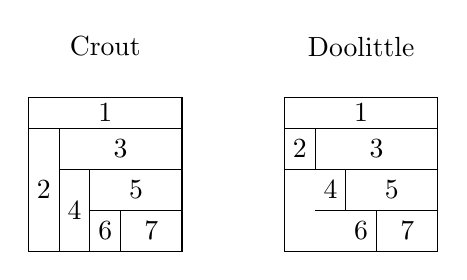
\begin{tikzpicture}[scale=.65]
\node at(1.5,4){Crout};\draw(0,0)rectangle(3,3);\draw(0,2.4)--(3,2.4);\draw(.6,0)--(.6,2.4);\draw(.6,1.6)--(3,1.6);\draw(1.2,0)--(1.2,1.6);\draw(1.2,.8)--(3,.8);\draw(1.8,0)--(1.8,.8);\node at(1.5,2.7){1};\node at(.3,1.2){2};\node at(1.8,2){3};\node at(.9,.8){4};\node at(2.1,1.2){5};\node at(1.5,.4){6};\node at(2.4,.4){7};
\begin{scope}[xshift=5cm]\node at(1.5,4){Doolittle};\draw(0,0)rectangle(3,3);\draw(0,2.4)--(3,2.4);\draw(0,1.6)--(3,1.6);\draw(0,0)--(0,2.4);\draw(.6,1.6)--(.6,2.4);\draw(.6,.8)--(3,.8);\draw(1.2,.8)--(1.2,1.6);\draw(1.2,0)--(3,0);\draw(1.8,0)--(1.8,.8);\node at(1.5,2.7){1};\node at(.3,2){2};\node at(1.8,2){3};\node at(.9,1.2){4};\node at(2.1,1.2){5};\node at(1.5,.4){6};\node at(2.4,.4){7};\end{scope}\end{tikzpicture}\end{center}
% Pagina originale 26
\pagina{26}
\begin{center}\begin{tabular}{c|l|l}Passo&Crout&Doolittle\\1&riga 1 di $U$&riga 1 di $U$\\2&riga 2 di $L$&colonna 1 di $L$\\3&riga 2 di $U$&riga 2 di $U$\\4&riga 3 di $L$&colonna 2 di $L$\\5&riga 3 di $U$&riga 3 di $U$\\&$\vdots$&$\vdots$\end{tabular}\end{center}
La matrice $U$ coincide con $A^{(n)}$, mentre in $L$ avremo i moltiplicatori. Nella tecnica di fattorizzazione LU non è semplice trovare una strategia di pivoting.
\subsection*{Equivalenza tra Gauss e fattorizzazione LU}
\[A\bar x=\bar b\Longrightarrow A^{(1)}\bar x=\bar b^{(1)}.\]
\[L^{(1)}=\begin{pmatrix}1&0&\cdots&0\\\ell_{21}&1&\cdots&0\\\vdots& &\ddots&\vdots\\\ell_{n1}&0&\cdots&1\end{pmatrix},\quad A^{(2)}=L^{(1)}A^{(1)},\quad\bar b^{(2)}=L^{(1)}\bar b^{(1)}.\]
Si dimostra in generale che $L^{(k)}A^{(k)}=A^{(k+1)}$ e $L^{(k)}\bar b^{(k)}=\bar b^{(k+1)}$, con $L^{(k)}$ uguale all'identità salvo la colonna $k$, che sotto la diagonale contiene $\ell_{k+1,k},\ldots,\ell_{nk}$.
\[A^{(n)}=L^{(n-1)}A^{(n-1)}=L^{(n-1)}L^{(n-2)}\cdots L^{(1)}A^{(1)},\quad\bar b^{(n)}=L^{(n-1)}\bar b^{(n-1)}.\]
L'inversa $(L^{(k)})^{-1}$ contiene $-\ell_{ik}$ al posto di $\ell_{ik}$.
\[L=(L^{(1)})^{-1}(L^{(2)})^{-1}\cdots(L^{(n-1)})^{-1}.\]
% Pagina originale 27
\pagina{27}
\[(L^{(1)})^{-1}\cdots(L^{(n-1)})^{-1}=(L^{(n-1)}\cdots L^{(1)})^{-1}=L.\]
\[\underbrace{(L^{(1)})^{-1}\cdots(L^{(n-1)})^{-1}}_L A^{(n)}=A,\quad A^{(n)}=U\Longrightarrow LU=A.\]
\[L=\begin{pmatrix}1&0&0&0\\-\ell_{21}&1&0&0\\-\ell_{31}&-\ell_{32}&1&0\\-\ell_{41}&-\ell_{42}&-\ell_{43}&1\end{pmatrix},\quad U=A^{(n)}.\]
\subsection*{Condizionamento di sistemi lineari}
\[\begin{cases}x+y=2\\1000x+1001y=2001\end{cases}\Longrightarrow x=y=1.\]
Perturbiamo $x$ dell'1\%: $\widetilde x=x(1+0.01)$.
\[\begin{cases}1.01x+y=2\\1000x+1001y=2001\end{cases}\Longrightarrow\widetilde x=-\frac19,\quad\widetilde y=\frac{1901}{900}.\]
\[\|\bar x-\widetilde{\bar x}\|=1.57=e_A(\bar x)=e_R(\bar x)\qquad\text{elevatissimo!}\]
\textit{Nota di trascrizione (pagina 27): uguaglianza degli errori riportata come nel manoscritto; norma non specificata.}
\[\widetilde A\widetilde{\bar x}=\widetilde{\bar b}\Longrightarrow(A+\delta A)(\bar x+\delta\bar x)=b+\delta b.\]
\[\frac{\|\delta\bar x\|}{\|\bar x\|}\le\underbrace{\|A\|\|A^{-1}\|}_{K}\left(\frac{\|\delta A\|}{\|A\|}+\frac{\|\delta b\|}{\|b\|}\right).\]
$K$ è detto indice di condizionamento del sistema.
% Pagina originale 28
\pagina{28}\section{Interpolazione}
È un metodo che consiste nell'approssimazione di una funzione dove conosciamo solo alcuni punti. L'insieme dei punti $x_i$ noti sono chiamati nodi. Certe volte è possibile interpolare una funzione anche se quest'ultima è nota ma è troppo complessa.
\[f(x)\simeq g(x;a_0,a_1,\ldots,a_n),\quad f(x_i)=g(x_i)\quad\forall i=0,\ldots,n.\]
Il procedimento più usato è quello nel quale
\[g(x;a_0,\ldots,a_n)=\sum_{i=0}^n a_i\phi_i(x),\quad f(x_j)=\sum_{i=0}^na_i\phi_i(x_j).\]
$g$ deve passare dai nodi. Risolvere quest'ultima equazione, trovando i coefficienti $a_i$, è il metodo dei coefficienti indeterminati.
\subsection*{Interpolazione polinomiale}
Con $\phi_i(x)=x^i$ per ogni $i$,
\[g(x;a_0,\ldots,a_n)=\sum_{i=0}^n a_ix^i,\]
è un polinomio. Le condizioni sono
\[a_0+a_1x_j+a_2x_j^2+\cdots+a_nx_j^n=f(x_j),\quad j=0,\ldots,n.\]
Sono riassumibili come $V\bar a=\bar y$, con
\[\bar y=(f(x_0),\ldots,f(x_n))^T,\quad\bar a=(a_0,\ldots,a_n)^T,\quad V=\begin{pmatrix}1&x_0&x_0^2&\cdots&x_0^n\\1&x_1&x_1^2&\cdots&x_1^n\\\vdots&\vdots&\vdots&&\vdots\\1&x_n&x_n^2&\cdots&x_n^n\end{pmatrix}\in\R^{(n+1)\times(n+1)}.\]
% Pagina originale 29
\pagina{29}
Se $V$ (matrice di Vandermonde) è non singolare il problema dell'interpolazione ammette un'unica soluzione. $V$ non è singolare se i nodi sono distinti a due a due. Risolvere il metodo dei coefficienti indeterminati richiede la soluzione di un sistema che potrebbe essere enorme e anche mal condizionato.
\subsection*{Polinomio interpolante di Lagrange}
\[L_n(x)=\sum_{k=0}^n\ell_{nk}(x)f(x_k),\]
con $\ell_{nk}(x)$ polinomio di grado $n$. Ponendo le condizioni $L_n(x_i)=f(x_i)$:
\[L_n(x_i)=\sum_{k=0}^n\ell_{nk}(x_i)f(x_k)=f(x_i)\Longrightarrow\ell_{nk}(x_i)=\begin{cases}0&k\ne i\\1&k=i.\end{cases}\]
Per far sì che il polinomio si annulli per $x_i$ con $i\ne k$, poniamo
\[\ell_{nk}(x)=c_k\prod_{\substack{i=0\\i\ne k}}^n(x-x_i),\quad \ell_{nk}(x_k)=c_k\prod_{\substack{i=0\\i\ne k}}^n(x_k-x_i)=1.\]
Quindi
\[c_k=\frac1{\prod_{i\ne k}(x_k-x_i)},\quad\boxed{L_n(x)=\sum_{k=0}^n\left(\prod_{\substack{i=0\\i\ne k}}^n\frac{x-x_i}{x_k-x_i}\right)f(x_k)}.\]
$\ell_{nk}(x)$ sono i polinomi fondamentali di Lagrange.
% Pagina originale 30
\pagina{30}\subsection*{Errori di interpolazione}
\[e(x)=f(x)-P_n(x).\]
$f(x)$ non è nota, quindi l'errore (o resto) dell'interpolazione non è direttamente calcolabile.
\subsection*{Teorema di rappresentazione dell'errore di interpolazione}
Sia $f\in C^{n+1}([a,b])$ e $x_i\in[a,b]$. Se $P_n(x)$ è il polinomio di interpolazione di $f(x)$ sui punti $x_i$, per ogni $x\in[a,b]$ esiste $\xi=\xi(x)$ tale che
\[e(x)=f(x)-P_n(x)=\frac{f^{(n+1)}(\xi)}{(n+1)!}(x-x_0)\cdots(x-x_n)=\frac{f^{(n+1)}(\xi)}{(n+1)!}\omega_{n+1}(x),\]
con $\omega_{n+1}(x)=\prod_{i=0}^n(x-x_i)$ polinomio nodale.
\textbf{Esempio.}
\[e(x)=f(x)-L_1(x)=\frac{f''(\xi_x)}{2!}(x-x_0)(x-x_1).\]
Ponendo $x=x_0+hs$, con $h=x_1-x_0$, $s\in[0,1]$, diventa
\begin{align*}e(x)&=\frac{f''(\xi_x)}2hs(x_0+hs-x_1)\\&=\frac{f''(\xi_x)}2hs(hs-h)=\frac{f''(\xi_x)}2h^2s(s-1)\\&=\frac{f''(x_0+\bar s h)}2h^2s(s-1).\end{align*}
\[\max_{s\in[0,1]}|s(s-1)|=\frac14\Longrightarrow |e(x)|\le\frac{h^2}8\max_{x\in[x_0,x_1]}|f''(x)|.\]
% Pagina originale 31
\pagina{31}\subsection*{Fenomeno di Runge}
\[f(x)=\frac1{1+x^2},\qquad x\in[-5,5],\qquad x_i=-5+\frac{10i}{n}.\]
$L_n(x)$ si allontana sempre più da $f(x)$ con $n\to+\infty$. Più suddivido l'intervallo $[a,b]$, più aumenta l'oscillazione e l'ampiezza.
\[\lim_{n\to\infty}\max_{x\in[-5,5]}|f(x)-L_n(x)|=+\infty.\]
Questo fenomeno è chiamato fenomeno di Runge ed è un grave problema dell'interpolazione di Lagrange.
\begin{center}\begin{tikzpicture}[x=0.5cm,y=2cm]\draw[->](-5.5,0)--(5.5,0);\draw[->](0,-.2)--(0,1.4);\draw[domain=-5:5,samples=80]plot(\x,{1/(1+\x*\x)})node[right]{$f$};\draw[dashed](-5,1.2)..controls(-4,-.3)and(-3,.3)..(-2,.2)..controls(0,1.8)and(1,.5)..(2,.2)..controls(3,-.2)and(4,.2)..(5,1.2)node[right]{$L_n$};\end{tikzpicture}\end{center}
\subsection*{Minimizzare il resto nel problema di interpolazione}
\[e(x)=\frac{f^{(n+1)}(\xi_x)}{(n+1)!}\omega_{n+1}(x).\]
Non possiamo modificare il fattore $f^{(n+1)}(\xi_x)/(n+1)!$, ma possiamo rendere $\omega_{n+1}(x)$ un polinomio di grado al più $n+1$ tale che
\[\max_{x\in[a,b]}|\widetilde p(x)|=\min_{p\in\mathcal P_{n+1}}\max_{x\in[a,b]}|p(x)|.\]
È fattibile utilizzando i polinomi di Chebyshev.
\textit{Nota (pagina 31): nel problema di minimo la famiglia deve intendersi monica, come il polinomio nodale; nel manoscritto questa restrizione non è esplicitata.}
\subsection*{Polinomio di Chebyshev}
\[T_n(x)=\cos(n\arccos x),\quad x\in[-1,1].\]
Esempio: $T_0(x)=\cos0=1$, $T_1(x)=x$.
% Pagina originale 32
\pagina{32}
Vale la seguente formula ricorsiva:
\[\boxed{T_{n+1}(x)=2xT_n(x)-T_{n-1}(x)}.\]
\textbf{Dimostrazione.} Posto $\arccos x=\theta$, $\cos\theta=x$:
\begin{align*}T_n(x)&=\cos(n\theta),\\T_{n+1}(x)&=\cos[(n+1)\theta]=\cos(n\theta)\cos\theta-\sin(n\theta)\sin\theta,\\T_{n-1}(x)&=\cos[(n-1)\theta]=\cos(n\theta)\cos\theta+\sin(n\theta)\sin\theta.\end{align*}
\[T_{n+1}(x)=2\cos(n\theta)\cos\theta-T_{n-1}(x)=2xT_n(x)-T_{n-1}(x).\]
\[T_0=1,\quad T_1=x,\quad T_2=2x\cdot x-1=2x^2-1,\quad T_3=2x(2x^2-1)-x=4x^3-3x.\]
Quindi $T_n(x)=2^{n-1}x^n+\cdots$.
\subsection*{Proprietà di $T_n$}
\begin{enumerate}\item $\max_{x\in[-1,1]}|T_n(x)|=1$.
\item $T_{2k}(-x)=T_{2k}(x)$ e $T_{2k+1}(-x)=-T_{2k+1}(x)$.
\item $|T_n(x)|=1$ per $x=\cos(k\pi/n)$. In particolare $T_n(x_k)=(-1)^k$, $k=0,\ldots,n$.
\item $T_n(x_k)=0$ per $x_k=\cos((2k+1)\pi/(2n))$, $k=0,\ldots,n-1$.\end{enumerate}
% Pagina originale 33
\pagina{33}\subsection*{Teorema di minimax}
Sia $p_n(x)$ un qualsiasi polinomio monico di grado $n$.
\[\frac1{2^{n-1}}=\max_{x\in[-1,1]}|\widehat T_n(x)|\le\max_{x\in[-1,1]}|p_n(x)|,\quad\widehat T_n(x)=\frac1{2^{n-1}}T_n(x).\]
$\widehat T_n$ è il polinomio di Chebyshev monico. In realtà il massimo di $|p_n|$ è maggiore di quello di $|\widehat T_n|$ (salvo coincidenza): il polinomio di Chebyshev monico è il polinomio di grado $n$ con il più piccolo dei massimi.
Ponendo $\omega_{n+1}(x)=\widehat T_{n+1}(x)$ avremo
\[|e(x)|=\left|\frac{f^{(n+1)}(\xi_x)}{(n+1)!}\widehat T_{n+1}(x)\right|\le\frac1{(n+1)!2^n}\max_{x\in[-1,1]}|f^{(n+1)}(x)|.\]
Se $[a,b]\ne[-1,1]$ bisogna effettuare una trasformazione lineare tra i due intervalli:
\[t=\frac{b-a}2x+\frac{a+b}2,\quad x\in[-1,1].\]
Detti $x_k$ gli zeri di $T_{n+1}(x)$,
\[\tau_k=\frac{b-a}2x_k+\frac{b+a}2,\quad k=0,\ldots,n,\quad x_k=\cos\frac{(2k+1)\pi}{2(n+1)}.\]
Usando gli zeri del polinomio di Chebyshev come nodi avremo il resto minimo (errore massimo). I nodi da usare sono dunque $\tau_k$, trasformati degli zeri di $\widehat T_{n+1}$.
% Pagina originale 34
\pagina{34}
Se il numero di nodi è sufficientemente elevato la funzione interpolante potrebbe mostrare un comportamento fortemente oscillatorio. A questo punto è preferibile usare l'approccio spline.
\subsection*{Funzioni spline}
\[\Delta:\quad a\equiv x_0<x_1<x_2<\cdots<x_n<x_{n+1}\equiv b\]
è una decomposizione dell'intervallo $[a,b]$. $s(x)$ è una funzione spline di grado $m\ge1$ relativa alla decomposizione $\Delta$ che ha le seguenti proprietà:
\begin{enumerate}\item $s|_{[x_i,x_{i+1}]}\in\mathcal P_m$.
\item $s^{(k)}(x)$ è continua in $[a,b]$ per ogni $k\in[0,m-1]$, cioè $s\in C^{m-1}$.\end{enumerate}
\subsection*{Approssimazione ai minimi quadrati}
\[\varepsilon_i=\phi(a_0,a_1,\ldots,a_m,x_i)-y_i,\quad i=0,1,\ldots,n,\]
è la differenza tra il valore assunto dalla funzione interpolante e la funzione effettiva nei nodi $y_i=f(x_i)$. Ricerchiamo $\bar a=(a_0,\ldots,a_m)$ tale che $\bar\varepsilon=(\varepsilon_0,\ldots,\varepsilon_n)$ abbia la minima norma euclidea al quadrato:
\[\|\bar\varepsilon\|_2^2=\sum_{i=0}^n\varepsilon_i^2=\sum_{i=0}^n\bigl(\phi(a_0,\ldots,a_m,x_i)-y_i\bigr)^2.\]
\[Q(a_0^*,\ldots,a_m^*)=\min_{a_0,\ldots,a_m\in\R}Q(a_0,\ldots,a_m),\quad Q=\|\bar\varepsilon\|_2^2.\]
Analizziamo il caso della retta $\phi(a_0,a_1,x)=\alpha x+\beta$.
% Pagina originale 35
\pagina{35}\subsection*{Retta di regressione}
\[\phi(\alpha,\beta,x)=\alpha x+\beta,\quad\alpha,\beta\in\R,\quad\phi(\alpha,\beta,x_i)-y_i=\alpha x_i+\beta-y_i.\]
\[\Psi(\alpha,\beta)=\sum_{i=0}^n(\alpha x_i+\beta-y_i)^2\quad\text{da minimizzare}.\]
\[\frac{\partial\Psi}{\partial\alpha}=\sum_{i=0}^n2x_i(\alpha x_i+\beta-y_i)=0,\quad\frac{\partial\Psi}{\partial\beta}=\sum_{i=0}^n2(\alpha x_i+\beta-y_i)=0.\]
\[\begin{cases}\alpha\sum x_i^2+\beta\sum x_i-\sum x_iy_i=0,\\\alpha\sum x_i+\beta\sum1-\sum y_i=0\end{cases}\Longrightarrow\begin{cases}\alpha\sum x_i^2+\beta\sum x_i=\sum x_iy_i,\\\alpha\sum x_i+\beta(n+1)=\sum y_i.\end{cases}\]
Posti $S_{xx}=\sum x_i^2$, $S_x=\sum x_i$, $S_y=\sum y_i$, $S_{xy}=\sum x_iy_i$:
\[\begin{cases}S_{xx}\alpha+S_x\beta=S_{xy},\\S_x\alpha+(n+1)\beta=S_y.\end{cases}\]
Usando Cramer:
\[\alpha=\frac{\begin{vmatrix}S_{xy}&S_x\\S_y&n+1\end{vmatrix}}{\begin{vmatrix}S_{xx}&S_x\\S_x&n+1\end{vmatrix}}=\frac{(n+1)S_{xy}-S_xS_y}{S_{xx}(n+1)-S_x^2},\]
\[\beta=\frac{\begin{vmatrix}S_{xx}&S_{xy}\\S_x&S_y\end{vmatrix}}{\begin{vmatrix}S_{xx}&S_x\\S_x&n+1\end{vmatrix}}=\frac{S_{xx}S_y-S_xS_{xy}}{S_{xx}(n+1)-S_x^2}.\]

% Pagina originale 36
\pagina{36}
\section*{Quadratura}
La quadratura è una tecnica che consente di calcolare
\[\int_a^b f(x)\,dx=I(f)\]
conoscendo $f(x)$ nell'intervallo $[a,b]$, quando diventa difficile o costoso calcolare $F(x)$ o quando si conoscono solo un certo numero di punti appartenenti ad $f(x)$.
\subsection*{Formule di quadratura di tipo interpolatorio}
\[\sum_{k=0}^m w_k f(x_k)\simeq I(f).\]
Formule di quadratura con $x_k$ nodi e $w_k$ pesi. Poniamo $f(x)=L_m(x)+e(x)$:
\begin{align*}
\int_a^b f(x)\,dx&=\int_a^b L_m(x)\,dx+\int_a^b e(x)\,dx\\
&=\int_a^b\sum_{k=0}^m\ell_{mk}(x)f(x_k)\,dx+\int_a^b e(x)\,dx\\
&=\sum_{k=0}^m\left[\int_a^b\ell_{mk}(x)\,dx\right]f(x_k)+\int_a^b e(x)\,dx.
\end{align*}
Pongo
\[w_k=\int_a^b\ell_{mk}(x)\,dx,\qquad R_{m+1}(f)=\int_a^b e(x)\,dx.\]
Le $\ell_{mk}$ sono le formule interpolatrici; $R_{m+1}(f)$ è il resto della formula di quadratura:
\[\boxed{I(f)=\sum_{k=0}^m w_k f(x_k)+R_{m+1}(f)},\qquad I(f)\simeq\sum_{k=0}^m w_k f(x_k).\]
\subsection*{Grado di precisione}
Una formula ha grado di precisione $q$ se fornisce il valore esatto di $I(f)$ quando $f$ è un polinomio di grado al più $q$ e $\exists p(x)\in\mathcal P_{q+1}\setminus\mathcal P_q$ tale che $R_{q+1}(f)\ne0$.
% Pagina originale 37
\pagina{37}
\textbf{Osservazione.} Ogni formula di quadratura di tipo interpolatorio ha grado di precisione $q\ge m$ ($m=\text{numero dei nodi}-1$).
\textbf{Dimostrazione.}
\[\int_a^b p_m(x)\,dx=\sum_{i=0}^m w_i p_m(x_i)+R_{m+1}(f),\]
\[R_{m+1}(f)=\int_a^b e(x)\,dx=\int_a^b\omega_{m+1}(x)\frac{p_m^{(m+1)}(x)}{(m+1)!}\,dx\equiv0,\]
poiché $p_m^{(m+1)}(x)=0$ per ogni $p_m\in\mathcal P_m$.
\subsection*{Formule di Newton--Cotes}
Suddivido $[a,b]$ in $m$ sottointervalli di ampiezza $h$, con
\[h=\frac{b-a}{m},\qquad x_i=a+ih,\quad i=0,1,\ldots,m.\]
\[\int_a^b f(x)\,dx=\sum_{i=0}^m w_i f(x_i)+R_{m+1}(f)\]
è la formula di Newton--Cotes.
\textbf{Proprietà:} $w_i=w_{m-i}$ (proprietà di simmetria).
\textbf{Dimostrazione.}
\[c=\frac{x_i+x_{m-i}}2=\frac{b+a}2\quad\Longrightarrow\quad
\begin{cases}x_i=2c-x_{m-i},\\x_{m-i}=2c-x_i.\end{cases}\]
\begin{align*}
w_k&=\int_a^b\prod_{\substack{i=0\\i\ne k}}^m\frac{x-x_i}{x_k-x_i}\,dx\\
&=\int_a^b\prod_{\substack{i=0\\i\ne k}}^m\frac{x-2c+x_{m-i}}{2c-x_{m-k}-2c+x_{m-i}}\,dx\\
&=\int_a^b\prod_{\substack{i=0\\i\ne k}}^m\frac{2c-x-x_{m-i}}{x_{m-k}-x_{m-i}}\,dx.
\end{align*}
Posto $t=2c-x$, si ha $t=2c-a=b$, $t=2c-b=a$, $dt=-dx$: si scambiano gli estremi di integrazione,
\[\int_a^b f(x)\,dx=-\int_b^a f(t)\,dt=\int_a^b f(t)\,dt.\]
Quindi
\[w_k=\int_a^b\prod_{\substack{i=0\\i\ne k}}^m\frac{t-x_{m-i}}{x_{m-k}-x_{m-i}}\,dt
=\int_a^b\prod_{\substack{j=0\\j\ne m-k}}^m\frac{t-x_j}{x_{m-k}-x_j}\,dt=w_{m-k},\qquad j=m-i.\]
% Pagina originale 38
\pagina{38}
\subsection*{Formula dei trapezi}
\[x_0=a,\quad x_1=b,\quad h=b-a,\qquad T_2=w_0f(x_0)+w_1f(x_1).\]
\begin{center}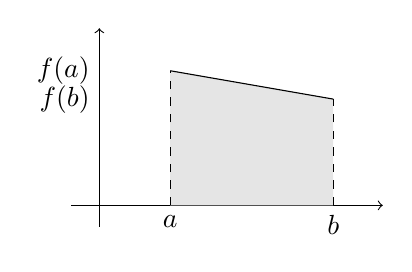
\begin{tikzpicture}[scale=.9]
\draw[->](-.4,0)--(4,0);\draw[->](0,-.3)--(0,2.5);
\fill[gray!20](1,0)--(1,1.9)--(3.3,1.5)--(3.3,0)--cycle;
\draw(1,1.9)--(3.3,1.5);\draw[dashed](1,0)--(1,1.9)(3.3,0)--(3.3,1.5);
\node[below]at(1,0){$a$};\node[below]at(3.3,0){$b$};\node[left]at(0,1.9){$f(a)$};\node[left]at(0,1.5){$f(b)$};
\end{tikzpicture}\end{center}
\begin{align*}
w_0&=\int_a^b\ell_{10}(x)\,dx=\int_a^b\frac{x-x_1}{x_0-x_1}\,dx
=\int_a^b\frac{x-b}{a-b}\,dx\\
&=\frac1{a-b}\left[\frac{(x-b)^2}2\right]_{x=a}^{x=b}
=-\frac{h^2}2\frac1{-h}=\frac h2.
\end{align*}
$a$ e $b$ sono nodi simmetrici rispetto a $c$, quindi $w_0=w_1=h/2$:
\[\boxed{T_2=\frac h2\bigl(f(a)+f(b)\bigr)}\qquad\text{formula dei trapezi}.\]
\subsection*{Resto nella formula dei trapezi}
\[R_2(f)=\frac1{2!}\int_a^b(x-a)(x-b)f''(\xi_x)\,dx.\]
Per manipolare quest'espressione abbiamo bisogno di conoscere il teorema della media generalizzato.
\subsection*{Teorema della media generalizzato}
Siano $f,g:[a,b]\to\mathbb R$, $f$ continua, $g(x)$ a segno costante e $g(x)\ne0$ per ogni $x\in(a,b)$. Allora
\[\int_a^b f(x)g(x)\,dx=f(\bar x)\int_a^b g(x)\,dx,\qquad\bar x\in[a,b].\]
Poiché $(x-a)(x-b)$ è a segno costante,
\[\int_a^b(x-a)(x-b)f''(\xi_x)\,dx=f''(\eta)\int_a^b(x-a)(x-b)\,dx\]
e quindi
\[R_2(f)=\frac{f''(\eta)}{2!}\int_a^b(x-a)(x-b)\,dx.\]
% Pagina originale 39
\pagina{39}
Posto $h=b-a$ e $x=a+ht$, con $t\in[0,1]$, $dx=h\,dt$:
\begin{align*}
R_2(f)&=\frac{f''(\eta)}{2!}\int_0^1 ht(-h+ht)h\,dt\\
&=\frac{f''(\eta)}{2!}\int_0^1 h^3t(t-1)\,dt
=\frac{f''(\eta)}{2!}h^3\left[\frac{t^3}3-\frac{t^2}2\right]_0^1
=-\frac{h^3}{12}f''(\eta).
\end{align*}
$R_2(f)=0\Longleftrightarrow f\in\mathcal P_1$. Il grado di precisione è $q=1$ (con $f$ di grado $2$, $R_2(f)\ne0$).
\subsection*{Formula di Simpson}
\[x_0=a,\quad x_2=b,\quad x_1=c=\frac{b+a}2,\qquad h=\frac{b-a}2,\]
\[S_3=w_0f(a)+w_1f(c)+w_2f(b).\]
\[w_0=\int_a^b\ell_{20}(x)\,dx=\int_a^b\frac{(x-b)(x-c)}{(a-b)(a-c)}\,dx.\]
Posto $x=c+ht$, $dx=h\,dt$:
\begin{align*}
w_0&=\int_{-1}^1\frac{(ht-h)(ht)}{(-2h)(-h)}h\,dt
=\int_{-1}^1\frac{(t-1)ht}2\,dt\\
&=\frac h2\left[\frac{t^3}3-\frac{t^2}2\right]_{-1}^1
=\frac h2\left(-\frac16+\frac56\right)=\frac23\frac h2=\frac h3.
\end{align*}
$w_0=w_2=h/3$ per simmetria.
\begin{align*}
w_1&=\int_a^b\ell_{21}(x)\,dx=\int_a^b\frac{(x-a)(x-b)}{(c-a)(c-b)}\,dx\\
&=\int_{-1}^1\frac{h(1+t)(ht-h)}{h(-h)}h\,dt
=h\int_{-1}^1(1-t^2)\,dt\\
&=h\left[t-\frac{t^3}3\right]_{-1}^1=h\left(\frac23+\frac23\right)=\frac43h.
\end{align*}
% Pagina originale 40
\pagina{40}
\[\boxed{S_3=\frac h3\bigl(f(a)+4f(c)+f(b)\bigr)}\qquad\text{formula di Simpson}.\]
\[\boxed{R_3(f)=-h^5\frac{f^{(4)}(\sigma)}{90}},\quad\sigma\in(a,b),\qquad h=\frac{b-a}2.\]
Grado di precisione $q=3$.
\subsection*{Formula del punto di mezzo}
Sia $c=(a+b)/2$. Sviluppo la serie di Taylor con $c$ punto iniziale:
\[f(x)=f(c)+f'(c)(x-c)+\frac{f''(\xi_x)}{2!}(x-c)^2,\qquad\xi_x\in[a,b].\]
\begin{align*}
\int_a^b f(x)\,dx&=\int_a^b f(c)\,dx+f'(c)\underbrace{\int_a^b(x-c)\,dx}_{0}
+\int_a^b\frac{f''(\xi)}2(x-c)^2\,dx\\
&=f(c)(b-a)+\int_a^b\frac{f''(\xi)}2(x-c)^2\,dx.
\end{align*}
Posto $h=b-a$, $\int_a^b f(x)\,dx\simeq hf(c)$.
\begin{align*}
R(f)&=\int_a^b\frac{f''(\xi)}2(x-c)^2\,dx
=\frac{f''(\eta)}2\int_a^b(x-c)^2\,dx\\
&=\frac{f''(\eta)}2\left.\frac{(x-c)^3}3\right|_a^b
=\frac{f''(\eta)}2\left(\frac{h^3}{24}+\frac{h^3}{24}\right)=\frac{h^3}{24}f''(\eta).
\end{align*}
\[\boxed{R(f)=\frac{h^3}{24}f''(\eta)},\qquad\boxed{M=hf(c)}.\]
Grado di precisione $q=1$. Il grado di precisione di questa tecnica è uguale a quello del trapezio, ma questa formula necessita solo di un punto.
\subsection*{Formule di quadratura composte}
Consiste nel dividere l'intervallo $[a,b]$ in $N$ sottointervalli con ampiezza uguale, aumentando la precisione.
% Pagina originale 41
\pagina{41}
\[\int_a^b f(x)\,dx=\sum_{i=0}^{N-1}\int_{x_i}^{x_{i+1}} f(x)\,dx,\quad x_i=a+ih,\quad h=\frac{b-a}N.\]
\subsection*{Formula dei trapezi composti}
\begin{align*}
\int_a^b f(x)\,dx&=\sum_{i=0}^{N-1}\left[\frac h2\bigl(f(x_i)+f(x_{i+1})\bigr)-\frac1{12}h^3f''(\eta_i)\right]\\
&=\frac h2\sum_{i=0}^{N-1}\bigl(f(x_i)+f(x_{i+1})\bigr)-\frac1{12}h^3\sum_{i=0}^{N-1}f''(\eta_i)\\
&=\frac h2\bigl(f(x_0)+f(x_N)\bigr)+h\sum_{i=1}^{N-1}f(x_i)-\frac{h^3}{12}Nf''(\eta),
\end{align*}
con $\eta_i\in(x_i,x_{i+1})$ e $\eta\in(a,b)$.
\[\boxed{T_c^{(h)}=\frac h2\bigl(f(x_0)+f(x_N)\bigr)+h\sum_{i=1}^{N-1}f(x_i)}.\]
\[R_T=-\frac{h^3}{12}Nf''(\eta)=-\frac{(b-a)^3}{12N^3}Nf''(\eta)
=\boxed{-\frac{(b-a)^3}{12N^2}f''(\eta)}.\]
Teorema della media nel discreto:
\[\sum_{i=1}^N f(x_i)=Nf(\bar x),\quad x_i\in[a,b],\quad\bar x\in(a,b).\]
Sappiamo che
\[|R_T|\le\frac1{12}\frac{(b-a)^3}{N^2}\underbrace{\max_{x\in(a,b)}|f''(x)|}_{M}.\]
\[\varepsilon\ge\frac1{12}\frac{(b-a)^3}{N_\varepsilon^2}M
\quad\Longrightarrow\quad N_\varepsilon\ge\sqrt{\frac{(b-a)^3M}{12\varepsilon}}.\]
Possiamo stabilire in quanti pezzi suddividere $[a,b]$ per ottenere una precisione $\varepsilon\ge|R_T|$.
\subsection*{Formula di Simpson composta}
Suddivido $[a,b]$ in $N$ intervalli, con $N$ pari:
\begin{align*}
\int_a^b f(x)\,dx&=\sum_{i=0}^{N/2-1}\int_{x_{2i}}^{x_{2i+2}}f(x)\,dx\\
&=\sum_{i=0}^{N/2-1}\left[\frac h3\bigl(f(x_{2i})+4f(x_{2i+1})+f(x_{2i+2})\bigr)-\frac{h^5}{90}f^{(4)}(\eta_i)\right].
\end{align*}
% Pagina originale 42
\pagina{42}
\[\int_a^b f(x)\,dx=\frac h3\sum_{i=0}^{N/2-1}\bigl[f(x_{2i})+4f(x_{2i+1})+f(x_{2i+2})\bigr]-\frac{h^5N}{180}f^{(4)}(\eta).\]
\[\boxed{S_c(h)=\frac h3\left[f(x_0)+f(x_N)+2\sum_{i=1}^{N/2-1}f(x_{2i})+4\sum_{i=0}^{N/2-1}f(x_{2i+1})\right]}.\]
\[R_S=-\frac{h^5N}{90}f^{(4)}(\eta)=-\boxed{\frac{(b-a)^5}{180N^4}f^{(4)}(\eta)}.\]
\emph{Nota di trascrizione (pagina 42): il denominatore 90 nella prima espressione di $R_S$ compare così nell'originale, mentre le espressioni adiacenti hanno 180.}
\[|R_S|\le\frac{(b-a)^5}{180N^4}\max_{x\in(a,b)}|f^{(4)}(x)|,\]
\[\varepsilon\ge\frac{(b-a)^5}{180N_\varepsilon^4}M\quad\Longrightarrow\quad
N_\varepsilon\ge\sqrt[4]{\frac{(b-a)^5M}{180\varepsilon}}.\]
\subsection*{Formula del punto di mezzo composta}
\begin{align*}
\int_a^b f(x)\,dx&=\sum_{i=0}^{N/2-1}\int_{x_{2i}}^{x_{2i+2}}f(x)\,dx\\
&=\sum_{i=0}^{N/2+1}2h f(x_{2i+1})+\sum_{i=0}^{N/2-1}\frac{(2h)^3}{24}f''(\eta_i)\\
&=2h\sum_{i=0}^{N/2+1}f(x_{2i+1})+\frac{h^3}{6}Nf''(\eta).
\end{align*}
\[\boxed{M_c(h)=2h\sum_{i=0}^{N/2-1}f(x_{2i+1})},\qquad
\boxed{R_M=\frac{(b-a)^3}{6N^2}f''(\eta)},\qquad N_\varepsilon\ge\sqrt{\frac{(b-a)^3M}{6\varepsilon}}.\]
\emph{Nota di trascrizione (pagina 42): gli indici $N/2+1$ delle due somme intermedie e il coefficiente del resto sono riprodotti come nella fonte; la formula evidenziata ha indice $N/2-1$.}
\section*{Derivazione numerica}
È una tecnica per trovare le derivate di una funzione senza calcolare effettivamente $f^{(m)}(t)$.
Supponiamo che $f\in C^k([a,b])$ con $k$ sufficientemente grande per i nostri scopi e dividiamo $[a,b]$ in
\[a\equiv t_0<t_1<t_2<\cdots<t_{N-1}<t_N\equiv b.\]
% Pagina originale 43
\pagina{43}
Considero tre punti consecutivi $t_{m-1},t_m,t_{m+1}$:
\[t_{m-1}=t_m-h,\qquad t_{m+1}=t_m+h.\]
\begin{align*}
f(t_{m+1})&=f(t_m)+f'(t_m)h+\frac{f''(t_m)}2h^2+\frac{f^{(3)}(t_m)}6h^3+\frac{f^{(4)}(\xi)}{24}h^4,\\
f(t_{m-1})&=f(t_m)-f'(t_m)h+\frac{f''(t_m)}2h^2-\frac{f^{(3)}(t_m)}6h^3+\frac{f^{(4)}(\eta)}{24}h^4.
\end{align*}
\[f(t_{m+1})+f(t_{m-1})=2f(t_m)+f''(t_m)h^2+\frac{h^4}{24}\bigl(f^{(4)}(\xi)+f^{(4)}(\eta)\bigr).\]
\[f(t_{m+1})+f(t_{m-1})\simeq2f(t_m)+f''(t_m)h^2\]
\[\boxed{f''(t_m)\simeq\frac{f(t_{m+1})+f(t_{m-1})-2f(t_m)}{h^2}}.\]
\[\boxed{E(f''(t_m))=-\frac{h^2}{24}\bigl(f^{(4)}(\xi)+f^{(4)}(\eta)\bigr)=-\frac{h^2}{12}f^{(4)}(\chi)},\quad\chi\in[t_{m-1},t_{m+1}].\]
Provo ad approssimare la derivata prima:
\begin{align*}
f(t_{m+1})&=f(t_m)+f'(t_m)h+\frac{f''(t_m)}2h^2+\frac{f^{(3)}(\sigma_1)}6h^3,\\
f(t_{m-1})&=f(t_m)-f'(t_m)h+\frac{f''(t_m)}2h^2-\frac{f^{(3)}(\sigma_2)}6h^3.
\end{align*}
\[f(t_{m+1})-f(t_{m-1})=2f'(t_m)h+\frac{f^{(3)}(\sigma)}3h^3.\]
\[\boxed{f'(t_m)\simeq\frac{f(t_{m+1})-f(t_{m-1})}{2h}}\qquad\text{formula delle differenze centrali}.\]
\[\boxed{E(f'(t_m))=-\frac{f^{(3)}(\delta)}6h^2},\qquad\delta\in[t_{m-1},t_{m+1}].\]
% Pagina originale 44
\pagina{44}
\subsection*{Differenze in avanti}
Sviluppo con Taylor $f(t_{m+1})$:
\[f(t_{m+1})=f(t_m)+hf'(t_m)+h^2\frac{f''(\sigma)}2\]
\[\boxed{f'(t_m)\simeq\frac{f(t_{m+1})-f(t_m)}h},\qquad
\boxed{E(f'(t_m))=-\frac h2 f''(\sigma)},\quad\sigma\in[t_m,t_{m+1}].\]
\subsection*{Differenze all'indietro}
Sviluppo con Taylor $f(t_{m-1})$:
\[f(t_{m-1})=f(t_m)-hf'(t_m)+h^2\frac{f''(\sigma)}2\]
\[\boxed{f'(t_m)\simeq\frac{f(t_m)-f(t_{m-1})}h},\qquad
\boxed{E(f'(t_m))=\frac h2 f''(\sigma)},\quad\sigma\in[t_{m-1},t_m].\]
\textbf{Nota.} Queste formule hanno ordine $1$ ($E\propto h$), mentre la formula delle differenze centrali ha ordine $2$ ($E\propto h^2$), quindi è più accurata.
\section*{Equazioni differenziali}
Definiamo un problema di Cauchy ai valori iniziali:
\[\begin{cases}y'(t)=f(t,y(t)),\\y(t_0)=y_0,\end{cases}\]
dove $f:[t_0,T]\times\mathbb R\to\mathbb R$, con $f\in C([t_0,T])$ e lipschitziana.
\textbf{Lipschitzianità.} $f$ è lipschitziana rispetto a $y$ se
\[\exists L>0:\quad\forall x,y\in\mathbb R:\quad|f(t,x)-f(t,y)|\le L|x-y|,\qquad\forall t\in[t_0,T].\]
% Pagina originale 45
\pagina{45}
$y(t)$ è soluzione dell'equazione differenziale se rispetta le condizioni del sistema ed è $y\in C^1([t_0,T])$.
Si discretizza l'intervallo di integrazione $[t_0,T]$:
\[t_{m+1}=t_m+h,\qquad t_m=t_0+mh,\quad m=0,1,\ldots,N,\qquad h=\frac{T-t_0}N.\]
\begin{align*}
y'(t)&=f(t,y(t))\\
\Longrightarrow\quad\int_{t_m}^{t_{m+1}}y'(t)\,dt&=\int_{t_m}^{t_{m+1}}f(t,y(t))\,dt\\
\Longrightarrow\quad y(t_{m+1})-y(t_m)&=\int_{t_m}^{t_{m+1}}f(t,y(t))\,dt.
\end{align*}
\subsection*{Metodo di Euler esplicito}
\[y(t_{m+1})-y(t_m)=hf(t_m,y(t_m))+\text{errore}\]
\[y(t_{m+1})-y(t_m)\simeq hf(t_m,y(t_m)).\]
Approssimo $y_{m+1}\simeq y(t_{m+1})$, $y_m\simeq y(t_m)$:
\[y_{m+1}-y_m=hf(t_m,y_m)\quad\Longleftrightarrow\quad
\boxed{y_{m+1}=y_m+hf(t_m,y_m)}.\]
È chiamato metodo di Euler esplicito in quanto, noto $y_m$, è possibile calcolare esplicitamente $y_{m+1}$.
\subsection*{Metodo di Euler implicito}
\[y(t_{m+1})-y(t_m)=hf(t_{m+1},y(t_{m+1}))+\text{errore}\]
\[y(t_{m+1})-y(t_m)\simeq hf(t_{m+1},y(t_{m+1}))\]
\[y_{m+1}-y_m\simeq hf(t_{m+1},y_{m+1})\quad\Longleftrightarrow\quad
\boxed{y_{m+1}=y_m+hf(t_{m+1},y_{m+1})}.\]
% Pagina originale 46
\pagina{46}\subsection*{Metodo dei trapezi}
\[y(t_{m+1})-y(t_m)\simeq\frac h2[f(t_m,y(t_m))+f(t_{m+1},y(t_{m+1}))].\]
\[\boxed{y_{m+1}=y_m+\frac h2[f(t_m,y_m)+f(t_{m+1},y_{m+1})]}.\]
\subsection*{Metodo del midpoint}
\[y(t_{m+2})-y(t_m)\simeq2hf(t_{m+1},y(t_{m+1})),\quad\boxed{y_{m+2}=y_m+2hf(t_{m+1},y_{m+1})}.\]
\begin{center}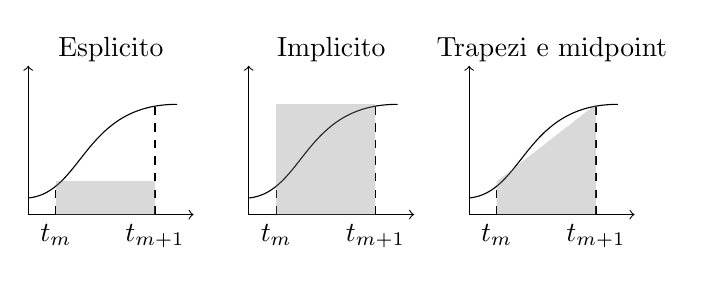
\begin{tikzpicture}[scale=.7]\foreach \d/\lab in {0/Esplicito,4/Implicito,8/Trapezi e midpoint}{\begin{scope}[xshift=\d cm]\draw[->](0,0)--(3,0);\draw[->](0,0)--(0,2.7);\draw(0,.3)..controls(1,.4)and(1,2)..(2.7,2);\draw[dashed](.5,0)node[below]{$t_m$}--(.5,.6)(2.3,0)node[below]{$t_{m+1}$}--(2.3,2);\node at(1.5,3){\lab};\end{scope}}\fill[gray,opacity=.3](.5,0)rectangle(2.3,.6);\fill[gray,opacity=.3](4.5,0)rectangle(6.3,2);\fill[gray,opacity=.3](8.5,0)--(8.5,.6)--(10.3,2)--(10.3,0)--cycle;\end{tikzpicture}\end{center}
\subsection*{Classificazione dei metodi numerici}
Se la soluzione nell'istante $t_{m+k}$ dipende da $k$ valori ottenuti in precedenza $t_{m+k-1},\ldots,t_{m+1},t_m$, il metodo si dice a $k$ passi ($k$-steps). Euler e trapezi sono a un passo (one-step); midpoint è a due passi.
\[y_{m+k}=y_m+h\Phi(t_m,\ldots,t_{m+k},y_m,\ldots,y_{m+k}),\]
\[y_{m+1}=y_m+h\Phi(t_m,t_{m+1},y_m,y_{m+1}).\]
Se $y_{m+1}=y_m+h\Phi(t_m,t_{m+1},y_m)$, o più in generale
\[y_{m+k}=y_m+h\Phi(t_m,\ldots,t_{m+k},y_m,\ldots,y_{m+k-1}),\]
il metodo è esplicito (Euler esplicito e midpoint).
% Pagina originale 47
\pagina{47}
Se ciò non fosse, il metodo è implicito (Euler implicito e trapezi). Per calcolare $y_{m+k}$ in un metodo implicito dovremo risolvere un'equazione che potrebbe non essere lineare se $f(t,y)$ non è lineare.
\[y_{m+1}=y_m+hf(t_{m+1},y_{m+1}),\qquad g(x)=y_m+hf(t_{m+1},x).\]
\[\boxed{y_{m+1}^{(r+1)}=g(y_{m+1}^{(r)})=y_m+hf(t_{m+1},y_{m+1}^{(r)})},\quad y_{m+1}^{(0)}=y_m.\]
Affinché il metodo converga $|g'(x)|<1$:
\[g'(x)=h\frac{\partial f}{\partial y}(t_{m+1},x),\quad\left|h\frac{\partial f}{\partial y}(t_{m+1},x)\right|<1\Longrightarrow h\left|\frac{\partial f}{\partial y}\right|<1\Longrightarrow\left|\frac{\partial f}{\partial y}\right|<\frac1h.\]
Questa condizione è verificata sicuramente perché $f(t,y)$ è lipschitziana, quindi $hL<1$.
\textit{Nota (pagina 47): la frase è riportata fedelmente; richiede che il passo sia scelto sufficientemente piccolo.}
Nel metodo di Euler esplicito
\[y=y_0+f(t_0,y_0)(t-t_0),\quad t=t_0+h\Longrightarrow y=y_0+hf(t_0,y_0)\Longrightarrow y_{k+1}=y_k+hf(t_k,y_k).\]
\begin{center}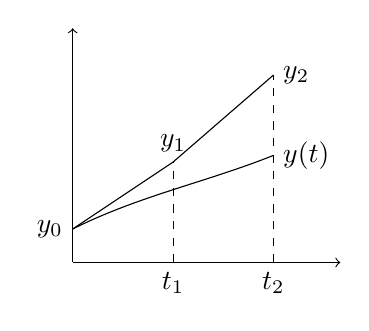
\begin{tikzpicture}[scale=.85]\draw[->](0,0)--(4,0);\draw[->](0,0)--(0,3.5);\draw(0,.5)..controls(1,1)and(2,1.2)..(3,1.6)node[right]{$y(t)$};\draw(0,.5)--(1.5,1.5)--(3,2.8)node[right]{$y_2$};\draw[dashed](1.5,0)node[below]{$t_1$}--(1.5,1.5)(3,0)node[below]{$t_2$}--(3,2.8);\node[left]at(0,.5){$y_0$};\node[above]at(1.5,1.5){$y_1$};\end{tikzpicture}\end{center}
% Pagina originale 48
\pagina{48}
Un altro metodo che coincide con il metodo di Euler esplicito consiste nel dividere in $N$ intervalli
\[t_0<t_1<t_2<\cdots<t_N\equiv T,\quad y'(t_m)=f(t_m,y_m)\simeq\frac{y_{m+1}-y_m}h\quad\text{(differenze in avanti)}.\]
Minore è $h$, più precisa sarà la soluzione. Il metodo è convergente se migliora l'approssimazione diminuendo opportunamente il passo $h$.
\subsection*{Studio della convergenza}
\[e(t_m,h):=y(t_m)-y_m\]
è l'errore globale. La convergenza consiste nell'annullarsi di $e(t_m,h)$ quando $h\to0$. Uno schema è convergente nel punto $T$ quando
\[\lim_{h\to0}e(t_m,h)=0\quad\Longleftrightarrow\quad\lim_{m\to+\infty}y_m=y(T).\]
Supponiamo di aver applicato Euler esplicito e indico con $y_m$ la soluzione approssimata. Chiamo $z(t)$ la soluzione dell'equazione differenziale che si ottiene prendendo $y_m$ come dato iniziale. Nella soluzione globale ci sono due errori:
\begin{enumerate}\item Errore di troncamento locale:
\[I_m(h,f):=z(t_{m+1})-[\underbrace{y_m}_{z(t_m)}+hf(t_m,y_m)].\]
Quest'errore è dovuto alla sostituzione della soluzione con la tangente.\end{enumerate}
% Pagina originale 49
\pagina{49}
\[\tau_m(h,f)=\frac{I_m(h,f)}h=\frac{z(t_m+h)-z(t_m)}h-f(t_m,z(t_m))\]
è chiamato errore di discretizzazione locale. Quando $\tau_m\to0$ per $h\to0$ il metodo è consistente.
\[\lim_{h\to0}\frac{z(t_m+h)-z(t_m)}h=z'(t_m)\Longrightarrow\lim_{h\to0}\tau_m(h,f)=z'(t_m)-f(t_m,z(t_m))=0,\]
perché $f(t_m,z(t_m))=z'(t_m)$. Quindi Euler esplicito è consistente.
Inoltre, espandendo $z(t_m+h)$ con Taylor:
\[z(t_m+h)=z(t_m)+hz'(t_m)+\frac{h^2}2z''(t_m+\theta h),\quad\theta\in(0,1).\]
Osservando $z'(t_m)=f(t_m,y_m)=f(t_m,z(t_m))$ si ha
\begin{align*}I_m(h,f)&=z(t_{m+1})-[y_m+hf(t_m,y_m)]\\&=z(t_m+h)-z(t_m)-hz'(t_m)=\frac{h^2}2z''(t_m+\theta h).\end{align*}
\[\boxed{\tau_m(h,f)=\frac{I_m(h,f)}h=\frac h2z''(t_m+\theta h)},\quad|\tau_m(h,f)|\le Mh,\quad M=\frac12\max_{\theta\in(0,1)}|z''(t_m+\theta h)|.\]
\textit{Nota (pagina 49): l'ultima riga manoscritta riporta $\tau(f,h)=O(h^2)$ e ``metodo di ordine $n$''; la pagina seguente precisa l'ordine corretto $1$.}
% Pagina originale 50
\pagina{50}
In questo caso $\tau(f,h)\propto h$, quindi $\tau=O(h^1)$: il metodo di Euler esplicito è di ordine 1.
\begin{enumerate}\setcounter{enumi}{1}\item Calcolo la tangente passante per il punto $(t_m,y_m)$ e non per $(t_m,y(t_m))$. Questo contributo non è locale in quanto rappresenta l'accumulo di tutti gli errori di troncamento locale commessi in precedenza.\end{enumerate}
Non è garantito che questi errori tendano a zero quando $h\to0$. In sintesi: non è detto che la convergenza a zero degli errori locali porti alla convergenza a zero dell'errore globale.
\[e(x)=0\quad\not\Longleftarrow\quad\tau_m(f,h)\to0\text{ con }h\to0\quad\forall m.\]
Il metodo è stabile se l'accumulo degli errori di troncamento locale si mantiene limitato per $h\to0$.
\[\boxed{\text{Convergenza}\quad\Longleftrightarrow\quad\text{Stabilità}+\text{Consistenza}}.\]

\end{document}
